% ---------------------------------------------------------------------------------------------------------------
% TEMPLATE EM LATEX PARA TRABALHO DE CONCLUSÃO DE CURSO DA URI ERECHIM
% (ESTE TEMPLATE NÃO É UM PROJETO OFICIAL DA URI) CONSULTE SEU ORIETADOR CASO QUEIRA UTILIZA-LO
% Este template foi baseado no template da Universidade Tecnológica Federal do Paraná UTFPR
%
% Template baseado no projeto: http://tcc.tsi.gp.utfpr.edu.br/paginas/modelos-latex-da-utfpr
%
%----------------------------------------------------------------------------------------------------------------
% Codificação: UTF-8
% LaTeX:  abnTeX2
% ---------------------------------------------------------------------------------------------------------------


% CARREGA CLASSE PERSONALIZADA COM AS NORMAS DA URI-----------------------------------------------------------
\documentclass[oneside]{template-config/uri-abntex2} %oneside -> impressão apenas frente

% INCLUI ARQUIVOS DE CONFIGURAÇÕES-------------------------------------------------------------------------------
% REFERÊNCIAS------------------------------------------------------------------
\usepackage[%
    alf,
    abnt-emphasize=bf,
    bibjustif,
    recuo=0cm,
    abnt-url-package=url,       % Utiliza o pacote url
    abnt-refinfo=yes,           % Utiliza o estilo bibliográfico abnt-refinfo
    abnt-etal-cite=3,
    abnt-etal-list=3,
    abnt-thesis-year=final
]{abntex2cite}                  % Configura as citações bibliográficas conforme a norma ABNT

% PACOTES----------------------------------------------------------------------
\usepackage[utf8]{inputenc}                                 % Codificação do documento
\usepackage[T1]{fontenc}                                    % Seleção de código de fonte
\usepackage{booktabs}                                       % Réguas horizontais em tabelas
\usepackage{color, colortbl}                                % Controle das cores
\usepackage{float}                                          % Necessário para tabelas/figuras em ambiente multi-colunas
\usepackage{graphicx}                                       % Inclusão de gráficos e figuras
\usepackage{icomma}                                         % Uso de vírgulas em expressões matemáticas
\usepackage{indentfirst}                                    % Indenta o primeiro parágrafo de cada seção
\usepackage{microtype}                                      % Melhora a justificação do documento
\usepackage{multirow, array}                                % Permite tabelas com múltiplas linhas e colunas
\usepackage{subeqnarray}                                    % Permite subnumeração de equações
\usepackage{lastpage}                                       % Para encontrar última página do documento
\usepackage{verbatim}                                       % Permite apresentar texto tal como escrito no documento, ainda que sejam comandos Latex
\usepackage{amsfonts, amssymb, amsmath}                     % Fontes e símbolos matemáticos
\usepackage[algoruled, portuguese]{algorithm2e}             % Permite escrever algoritmos em português
%\usepackage[scaled]{helvet}                                % Usa a fonte Helvetica
\usepackage{times}                                          % Usa a fonte Times
%\usepackage{palatino}                                      % Usa a fonte Palatino
%\usepackage{lmodern}                                       % Usa a fonte Latin Modern
\usepackage[bottom]{footmisc}                               % Mantém as notas de rodapé sempre na mesma posição
\usepackage{ae, aecompl}                                    % Fontes de alta qualidade
\usepackage{latexsym}                                       % Símbolos matemáticos
\usepackage{lscape}                                         % Permite páginas em modo "paisagem"
%\usepackage{picinpar}                                      % Dispor imagens em parágrafos
%\usepackage{scalefnt}
\usepackage{setspace}                                    % Permite redimensionar tamanho da fonte
%\usepackage{subfig}                                        % Posicionamento de figuras
%\usepackage{upgreek}                                       % Fonte letras gregas

% Redefine a fonte para uma fonte similar a Arial (fonte Helvetica)
% \renewcommand*\familydefault{\sfdefault}
% Configura todo o documento para times new roman
\renewcommand{\familydefault}{ptm}

% CONFIGURAÇÕES DE APARÊNCIA DO PDF FINAL--------------------------------------
\makeatletter
\hypersetup{%
    portuguese,
    colorlinks=true,   % true: "links" coloridos; false: "links" em caixas de texto
    linkcolor=black,    % Define cor dos "links" internos
    citecolor=black,    % Define cor dos "links" para as referências bibliográficas
    filecolor=black,    % Define cor dos "links" para arquivos
    urlcolor=black,     % Define a cor dos "hiperlinks"
    breaklinks=true,
    pdftitle={\@title},
    pdfauthor={\@author},
    pdfkeywords={abnt, latex, abntex, abntex2}
}
\makeatother

% ALTERA O ASPECTO DA COR AZUL--------------------------------------------------
\definecolor{blue}{RGB}{41,5,195}

% REDEFINIÇÃO DE LABELS---------------------------------------------------------
\renewcommand{\algorithmautorefname}{Algoritmo}
\def\equationautorefname~#1\null{Equa\c c\~ao~(#1)\null}

% CRIA ÍNDICE REMISSIVO---------------------------------------------------------
\makeindex

% HIFENIZAÇÃO DE PALAVRAS QUE NÃO ESTÃO NO DICIONÁRIO---------------------------
\hyphenation{%
    qua-dros-cha-ve
    Kat-sa-gge-los
}



% INCLUI ARQUIVOS DO TRABALHO DE CONCLUSÃO DE CURSO (PRÉ-TEXTUAIS, TEXTUAIS, PÓS-TEXTUAIS)-----------------------

% INSERE CAPA E FOLHA DE ROSTO
% CAPA---------------------------------------------------------------------------------------------------

% ORIENTAÇÕES GERAIS-------------------------------------------------------------------------------------
% Caso algum dos campos não se aplique ao seu trabalho, como por exemplo,
% se não houve coorientador, apenas deixe vazio.
% Exemplos: 
% \coorientador{}
% \departamento{}

% DADOS DO TRABALHO--------------------------------------------------------------------------------------
\titulo{Título do Trabalho: Subtítulo do Trabalho}
% \titleabstract{Title in English}
\autor{Nome Completo do Autor}
% \autorcitacao{SOBRENOME, Nome} % Sobrenome em maiúsculo
\local{ERECHIM - RS}
\data{2018}

% NATUREZA DO TRABALHO-----------------------------------------------------------------------------------
% Opções: 
% - Projeto de Conclusão de Curso (Disciplina de Projeto)
% - Trabalho de Conclusão de Curso (se for Graduação)
% - Dissertação (se for Mestrado)
% - Tese (se for Doutorado)
% - Projeto de Qualificação (se for Mestrado ou Doutorado)
% \projeto{Trabalho de Conclusão de Curso}

% TÍTULO ACADÊMICO---------------------------------------------------------------------------------------
% Opções:
% - Bacharel ou Tecnólogo (Se a natureza for Trabalho de Conclusão de Curso)
% - Mestre (Se a natureza for Dissertação)
% - Doutor (Se a natureza for Tese)
% - Mestre ou Doutor (Se a natureza for Projeto de Qualificação)
% \tituloAcademico{Bacharel}

% ÁREA DE CONCENTRAÇÃO E LINHA DE PESQUISA---------------------------------------------------------------
% Se a natureza for Trabalho de Conclusão de Curso, deixe ambos os campos vazios
% Se for programa de Pós-graduação, indique a área de concentração e a linha de pesquisa
% \areaconcentracao{}
% \linhapesquisa{}

% DADOS DA INSTITUIÇÃO-----------------------------------------------------------------------------------
% Se a natureza for Trabalho de Conclusão de Curso, coloque o nome do curso de graduação em "programa"
% Formato para o logo da Instituição: \logoinstituicao{<escala>}{<caminho/nome do arquivo>}
% \instituicao{Universidade Regional Integrada do Alto Uruguai e das Missões Campus de Erechim}
% \departamento{Departamento de Engenharias e Ciência da Computação}
% \programa{Curso de Ciência da Computação}
% \disciplina{Projeto de Conclusão de Curso}
%\logoinstituicao{0.2}{dados/figuras/logo-instituicao.png} 

% DADOS DOS ORIENTADORES---------------------------------------------------------------------------------
% \orientador{Nome do orientador}
%\orientador[Orientadora:]{Nome da orientadora}
% \instOrientador{Instituição do orientador}

% \coorientador{Nome do coorientador}
%\coorientador[Coorientadora:]{Nome da coorientadora}
% \instCoorientador{Instituição do coorientador}

% FOLHA DE ROSTO--------------------------------------------------------------------------------------------------------

% Os dados podem ser alterados em /text-elements/pre-textuais/capa.tex

% PROJETO DE CONCLUSÂO DE CURSO
% \preambulo{{\imprimirprojeto} elaborado e apresentado na disciplina de {\imprimirdisciplina}, Curso de {\imprimirprograma}, {\imprimirdepartamento} da {\imprimirinstituicao}.}

% TRABALHO DE CONCLUSÃO DE CURSO
\preambulo{{\imprimirprojeto} apresentado como requisito parcial à obtenção do grau de {\imprimirtituloAcademico}, {\imprimirdepartamento} da {\imprimirinstituicao}.}

% DISSERTAÇÃO DE MESTRADO
% \preambulo{{\imprimirprojeto} apresentada ao Programa de \mbox{Pós-graduação} da {\imprimirinstituicao}, como requisito parcial para obtenção do título de {\imprimirtituloAcademico}.}

% TESE DE DOUTORADO
% \preambulo{{\imprimirprojeto} apresentada ao Programa de \mbox{Pós-graduação} da {\imprimirinstituicao}, como requisito parcial para a obtenção do título de {\imprimirtituloAcademico}.}

% PROJETO DE QUALIFICAÇÃO DE MESTRADO OU DOUTORADO
%\preambulo{{\imprimirprojeto} apresentado ao Programa de \mbox{Pós-graduação} da {\imprimirinstituicao}, como requisito parcial para a obtenção do título de {\imprimirtituloAcademico}.}

% OBSERVAÇÕES-----------------------------------------------------------------------------------------------------------
% Altere este arquivo APENAS comentando as linhas que não se aplicam ao tipo de trabalho acadêmico desejado.

% \include{text-elements/pre-textuais/folha-aprovação}

\begin{document}

\pretextual
\imprimircapa                                               	           % Comando para imprimir Capa
\imprimirfolhaderosto{}                                     		   % Comando para imprimir Folha de rosto
% \imprimirfolhadeaprovacao
% INSERE ELEMENTOS PRÉ-TEXTUAIS
% DEDICATÓRIA------------------------------------------------------------------

\renewcommand{\dedicatorianame}{DEDICATÓRIA}

\begin{dedicatoria}

Altere este texto inserindo a dedicatória do seu trabalho. 

\end{dedicatoria}
          			   % Dedicatória
% AGRADECIMENTOS---------------------------------------------------------------

\begin{agradecimentos}[AGRADECIMENTOS]

Edite e coloque aqui os agradecimentos às pessoas e/ou instituições que contribuíram para a realização do trabalho.

É obrigatório o agradecimento às instituições de fomento à pesquisa que financiaram total ou parcialmente o trabalho, inclusive no que diz respeito à concessão de bolsas.

\end{agradecimentos}
        			   % Agradecimentos
% EPÍGRAFE---------------------------------------------------------------------

\renewcommand{\epigraphname}{EPÍGRAFE}

\begin{epigrafe}

\textit{Eu denomino meu campo de Gestão do Conhecimento, mas você não pode gerenciar conhecimento. Ninguém pode. O que pode fazer - o que a empresa pode fazer - é gerenciar o ambiente que otimize o conhecimento. (PRUSAK, Laurence, 1997).}

\end{epigrafe}

% OBSERVAÇÕES------------------------------------------------------------------
% Altere o texto para inserir a epígrafe do seu trabalho
              			   % Epígrafe
% RESUMO--------------------------------------------------------------------------------

\begin{resumo}[RESUMO]
\begin{SingleSpacing}

% Não altere esta seção do texto--------------------------------------------------------
\imprimirautorcitacao. \imprimirtitulo. \imprimirdata. \pageref {LastPage} f. \imprimirprojeto\ – \imprimirprograma, \imprimirinstituicao. \imprimirlocal, \imprimirdata.\\
%---------------------------------------------------------------------------------------

O Resumo é um elemento obrigatório em tese, dissertação, monografia e TCC, constituído de uma seqüência de frases concisas e objetivas, fornecendo uma visão rápida e clara do conteúdo do estudo. O texto deverá conter no máximo 500 palavras e ser antecedido
pela referência do estudo. Também, não deve conter citações. O resumo deve ser redigido em parágrafo único, espaçamento simples e seguido das palavras representativas do conteúdo do estudo, isto é, palavras-chave, em número de três a cinco, separadas entre si por ponto e finalizadas também por ponto. Usar o verbo na terceira pessoa do singular, com linguagem impessoal, bem como fazer uso, preferencialmente, da voz ativa. Texto contendo um único parágrafo.\\

\textbf{Palavras-chave}: Palavra. Segunda Palavra. Outra palavra.

\end{SingleSpacing}
\end{resumo}

% OBSERVAÇÕES---------------------------------------------------------------------------
% Altere o texto inserindo o Resumo do seu trabalho.
% Escolha de 3 a 5 palavras ou termos que descrevam bem o seu trabalho 
             			   % Resumo em Português
% ABSTRACT--------------------------------------------------------------------------------

\begin{resumo}[ABSTRACT]
\begin{SingleSpacing}

% Não altere esta seção do texto--------------------------------------------------------
\imprimirautorcitacao. \imprimirtitleabstract. \imprimirdata. \pageref {LastPage} f. \imprimirprojeto\ – \imprimirprograma, \imprimirinstituicao. \imprimirlocal, \imprimirdata.\\
%---------------------------------------------------------------------------------------

Elemento obrigatório em tese, dissertação, monografia e TCC. É a versão do resumo em português para o idioma de divulgação internacional. Deve ser antecedido pela referência do estudo. Deve aparecer em folha distinta do resumo em língua portuguesa e seguido das palavras representativas do conteúdo do estudo, isto é, das palavras-chave. Sugere-se a elaboração do resumo (Abstract) e das palavras-chave (Keywords) em inglês; para resumos em outras línguas, que não o inglês, consultar o departamento / curso de origem.\\

\textbf{Keywords}: Word. Second Word. Another word.

\end{SingleSpacing}
\end{resumo}

% OBSERVAÇÕES---------------------------------------------------------------------------
% Altere o texto inserindo o Abstract do seu trabalho.
% Escolha de 3 a 5 palavras ou termos que descrevam bem o seu trabalho 
             		           % Resumo em Inglês
% Lista de Figuras----------------------------------------------------------------

\pdfbookmark[0]{\listfigurename}{lof}
\listoffigures*
\cleardoublepage

% OBSERVAÇÕES---------------------------------------------------------------------
% Este arquivo não precisa de ser alterado, pois a lista é gerada automaticamente.
   % Lista de Figuras
% LISTA DE QUADROS----------------------------------------------------------------

\renewcommand{\listofquadrosname}{LISTA DE QUADROS}

\pdfbookmark[0]{\listofquadrosname}{loq}
\listofquadros*
\cleardoublepage

% OBSERVAÇÕES---------------------------------------------------------------------
% Este arquivo não necessita de ser editado. A lista é gerada automaticamente.
   % Lista de Quadros
% LISTA DE TABELAS-------------------------------------------------------------

\pdfbookmark[0]{\listtablename}{lot}
\listoftables*
\cleardoublepage

% OBSERVAÇÕES-------------------------------------------------------------------
% Este arquivo não precisa ser alterado, pois a lista é gerada automaticamente.
         		   % Lista de Tabelas
% LISTA DE ABREVIATURAS E SIGLAS----------------------------------------------------------

\begin{siglas}
    \item[ABNT] Associação Brasileira de Normas Técnicas
    \item[DECOM] Departamento de Computação
\end{siglas}

% OBSERVAÇÕES-----------------------------------------------------------------------------
% Altere a lista acima para definir os acrônimos e siglas utilizados neste trabalho
          		   % Lista de Abreviaturas e Siglas
% LISTA DE SÍMBOLOS------------------------------------------------------------

\begin{simbolos}
    \item[$ \Gamma $] Letra grega Gama
    \item[$ \lambda $] Comprimento de onda
    \item[$ \in $] Pertence
\end{simbolos}

% OBSERVAÇÕES-------------------------------------------------------------------
% Altere a lista acima para definir os símbolos utilizados no trabalho
        		   % Lista de Símbolos
% LISTA DE ALGORITMOS----------------------------------------------------------

\newcommand{\algoritmoname}{Algoritmo}
\renewcommand{\listalgorithmcfname}{LISTA DE ALGORITMOS}

\floatname{algocf}{\algoritmoname}
\newlistof{listofalgoritmos}{loa}{\listalgoritmoname}
\newlistentry{algocf}{loa}{0}

\counterwithout{algocf}{chapter}
\renewcommand{\cftalgocfname}{\algoritmoname\space}
\renewcommand*{\cftalgocfaftersnum}{\hfill--\hfill}

\pdfbookmark[0]{\listalgorithmcfname}{loa}
\listofalgorithms
\cleardoublepage

% OBSERVAÇÕES------------------------------------------------------------------
% Este arquivo não precisa ser alterado, pois a lista é gerada automaticamente.
   % Lista de Algoritmos
% SUMÁRIO----------------------------------------------------------------------

\renewcommand{\contentsname}{SUMÁRIO}

\pdfbookmark[0]{\contentsname}{toc}
\tableofcontents*
\cleardoublepage               			   % Sumário

\textual
% INSERE ELEMENTOS TEXTUAIS
% INTRODUÇÃO-------------------------------------------------------------------

\chapter{INTRODUÇÃO}
\label{chap:introducao}

\LaTeX{} é um conjunto de macros de alto nível para \TeX \xspace que torna mais fácil e rápida a produção de todo o tipo de documentos como, por exemplo, livros, relatórios e artigos.

O objetivo do \LaTeX \xspace é que o autor se possa distanciar da apresentação visual do trabalho e assim se concentrar no seu conteúdo. Possui formas de lidar com bibliografias, citações, formatos de páginas, referências e tudo mais que não seja relacionado com conteúdo do documento em si.

\section{Histórico}
\label{sec:Histórico}

Em 1978 Donald E. Knuth começou a desenvolver uma linguagem cujo objetivo era permitir a qualquer um formatar textos com muitas equações e com alta qualidade de saída, chamada de \TeX. Em 1985 Leisle Lamport desenvolveu um conjunto de macros denominado \LaTeX \xspace, que simplifica o uso da linguagem \TeX \xspace. Atualmente este projeto é mantido e desenvolvido pelo \LaTeX3 \xspace Project

O som final dos nomes \TeX \xspace e \LaTeX \xspace deve ser pronunciado como se fosse um “K”.

\section{Instalação}
\label{sec:Instalação}

\LaTeX é um software livre e gratuito, é possível instalar nos  principais sistemas operacionais modernos como: Windows 7, 8, 8.1 e 10; Mac OS e várias distribuições Linux.

\subsection{Windows}

MiKTeX é uma distribuição TeX / LaTeX para o Microsoft Windows. Baixe o instalador pelo link oficial: \href{https://miktex.org/download}{\textcolor{blue}{Download MiKTeX}}

A instalação do MiKTeX é simples, basicamente é só clicar no “Avançar”. Caso houver problemas na instalação o seguinte vídeo poderá servir de ajuda: \href{https://www.youtube.com/watch?v=4udFXbqtayE&list=LLQVoeslEpxQJ0UavpXUEkq}{\textcolor{blue}{Vídeo Instalação MiKTeX}}. Junto com a instalação do MiKTeX o editor TeXworks é instalado. Existem outros editores como o Texmaker. 

O Texmaker é mais simples de usar e é o editor de código aberto mais popular entre a comunidade LaTeX. Baixe o instalador pelo link oficial: \href{http://www.xm1math.net/texmaker/download.html}{\textcolor{blue}{Download TeXMaker}}

\subsection{Ubuntu}

O TeX Live é uma distribuição para produção de documentos \TeX \xspace. Para instalar no ubuntu 16.04 digite o seguinte comando: 
\begin{lstlisting}[language=bash]
    $ sudo apt-get install texlive-full
\end{lstlisting}

Apos a instalação do TeX Live pode-se obtar por instalar um editor específico para LaTeX o Texmaker, para instalar digite o seguinte comando: 

\begin{lstlisting}[language=bash]
    $ sudo apt-get install texmaker
\end{lstlisting}

\section{Compilação Tex Maker}

Para Compilar o arquivo \emph{.tex} junto com o arquivo \emph{.bib} no TeX Maker é necessário uma configuração, como mostra as Figuras \ref{fig:texmaker-config1} e \ref{fig:texmaker-config2}.

\begin{figure}[H]
    \centering
    \caption{Configuração Tex Maker}
    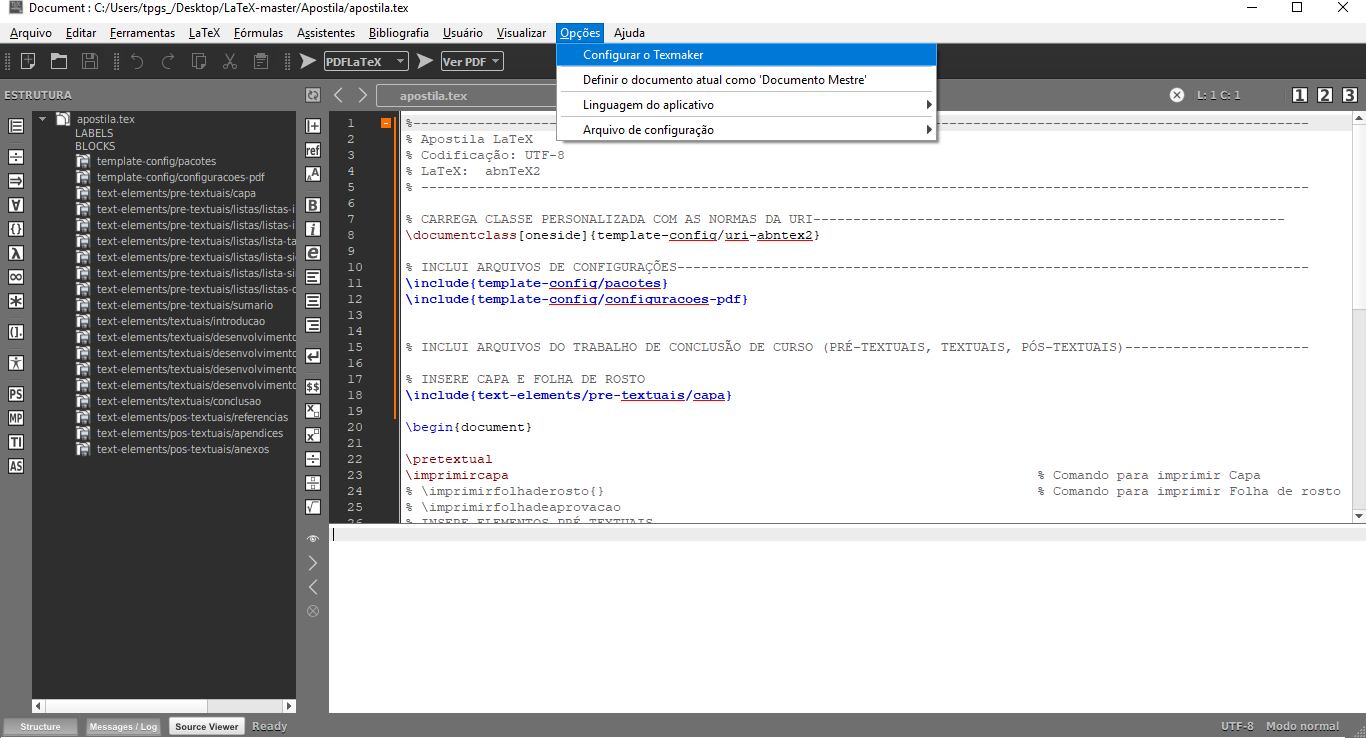
\includegraphics[width=0.70\textwidth]{./dados/figuras/compiler1}
    \fonte{Autor}
    \label{fig:texmaker-config1}
\end{figure}

\begin{figure}[H]
    \centering
    \caption{Configuração Tex Maker 2}
    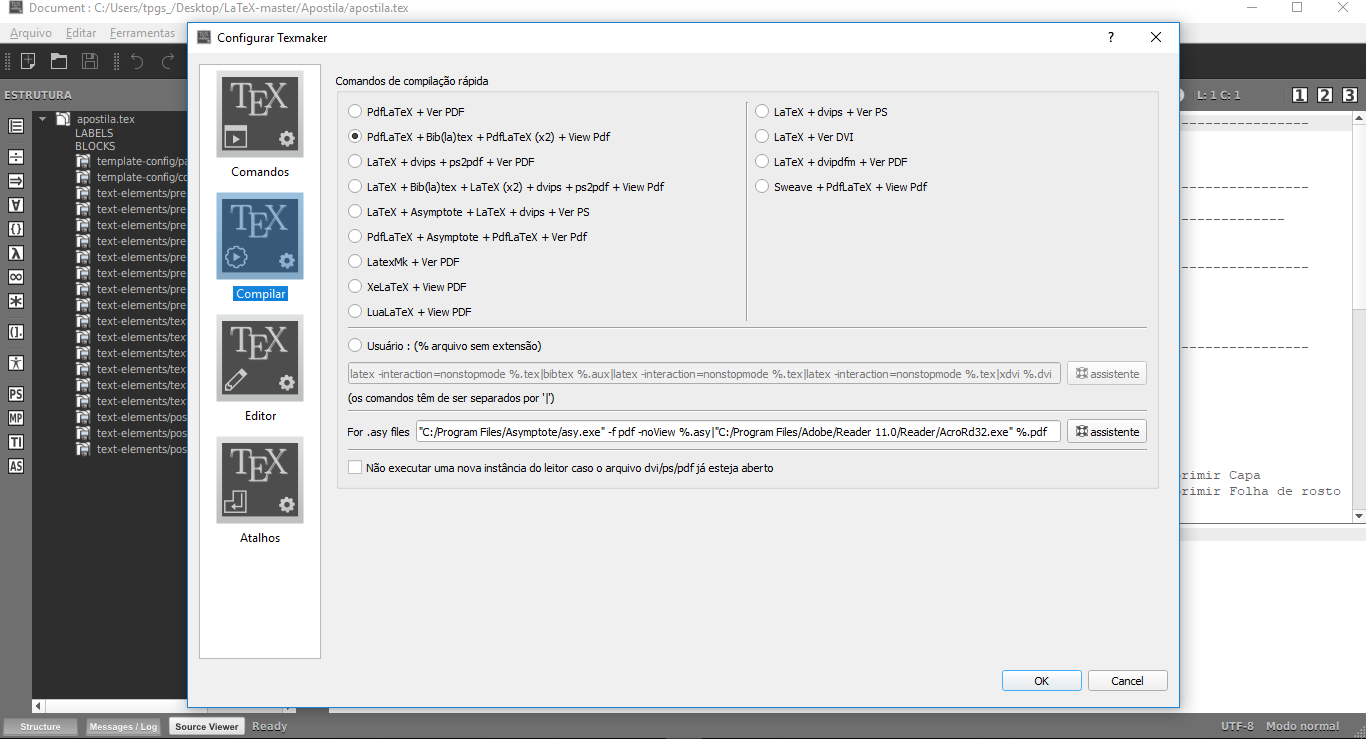
\includegraphics[width=0.70\textwidth]{./dados/figuras/compiler2}
    \fonte{Autor}
    \label{fig:texmaker-config2}
\end{figure}

\section{Compilação por Linha de Comando}

Para compilar pela linha de comando (windows e Linux) deve-se fazer os seguintes passos:

\begin{enumerate}
    \item Compilar o arquivo principal \emph{.tex}:
    \begin{lstlisting}[language=bash]
        pdflatex apostila.tex
    \end{lstlisting}
    \item Montar os índices:
    \begin{lstlisting}[language=bash]
        makeindex apostila.idx
    \end{lstlisting}
    \item Compilar o arquivo das bibliografias \emph{.bib}
    \begin{lstlisting}[language=bash]
        bibtex apostila.aux
    \end{lstlisting}
    \item Por fim, gerar o PDF:
    \begin{lstlisting}[language=bash]
        pdflatex apostila.tex
    \end{lstlisting}
\end{enumerate}

\section{Ferramentas em Nuvem}

Existem ferramentas que possibilitam a edição e a colaboração online de documentos LaTeX. Uma dessas ferramentas é o \href{https://www.overleaf.com/}{\textcolor{blue}{Overleaf}}.

Para usar o Overleaf basta criar uma conta, começar um projeto e escrever. Uma outra grande vantagem do Overleaf é a comunidade que compartilha templates prontos, como por exemplo:  \href{https://www.overleaf.com/latex/templates}{\textcolor{blue}{principais templates}}.                 		           % Introdução
% METODOLOGIA------------------------------------------------------------------

\chapter{PESQUISA}

  Como requerimento da introdução dos conceitos propostos neste trabalho, é necessário estabelecer uma base cuja será usada para solidificar a progressão da forma como são organizadas as abstrações apresentadas. Com a intenção da elaboração um modelo de estruturação de procedimentos, primeiro é indispensável definir o modelo de como é tradicionalmente estruturado um conjunto de informações para, então, explorar as possíveis formas de aumentar seu desempenho através de paralelização.
  
  \section{Estruturas de Dados}
  
  Em estruturas de dados convencionais, a tarefa proposta é modelar uma informação de forma que as relações entre os valores sejam claras e que o seu acesso seja eficiente. Cada estrutura de dado tem seus pontos fortes e fracos, e, por causa disso, é importante saber em quais situações cada uma delas será mais apropriada \cite{cormen2009}. Com esta concepção formalizada, apresenta-se a viabilidade do uso do mesmo conceito para modelar procedimentos ao invés de informações, e usar estes como blocos de construção para a criação de um processo maior, completamente personalizado para as necessidades que um desenvolvedor possa estar buscando atender.
  
  \section{\textit{Pipelining}}
  
  Uma técnica de computação paralela muito utilizada em linguagens com suporte a CSP (\textit{Communicating Sequential Processes}) é a de \textit{pipelining}. Uma \textit{pipeline} é uma série de estágios cuja entrada é a saída do anterior. Em cada um, o valor é recebido, algum tipo de processamento é realizado no mesmo e então ele é repassado para uma saída, onde será capturado pelo próximo ou pelo consumidor \cite{ajmani2014}. Na figura \ref{fig:stage} está sua representação: o losango representa a entrada, a flecha, a saída, e a linha entre os dois, a operação que é feita sobre os dados.
  
\begin{figure}[!htb]
    \centering
    \caption{Representação de um estágio do conceito de \textit{pipelining}}
    
\includegraphics[width=0.5\textwidth]{./dados/figuras/stage.png}
    \fonte{\citeonline{ajmani2014}}
    \label{fig:stage}
\end{figure}
  
A entrada do primeiro estágio é chamada de produtor, enquanto a saída do último é conhecida como consumidor \cite{ajmani2014}. O que garante o aspecto paralelo a esta técnica é que cada estágio pode ser executado em uma \textit{thread} própria, tendo um funcionamento similar à técnica de computação paralela conhecida por \textit{worker pool}, sendo que cada estágio pode ser considerado um \textit{worker}. A representação de uma pipeline é feita na figura \ref{fig:stage}, onde a flecha antecedendo o primeiro estágio simboliza o produtor, e o losango que sucede o último estágio, o consumidor.
  
  \section{Cuidados com a GPU}

  As características que mais influenciam a resistência de um processador são as que ressaltam a física dele.
  Por exemplo: O CPU tem IHS e o GPU não, esse já é um ponto a mais para o CPU na questão de resistência, 
  pois o GPU não tendo IHS, terá o núcleo exposto e consequentemente será mais sensível.
  Só que o GPU aguenta mais calor do que o CPU,entretanto ele ainda consome mais \textit{watts}.

  \begin{table}[h!]
    \centering
    \caption{Comparativo CPU X GPU}
    \label{comparativo}
    \begin{tabular}{|l|l|}
      \hline
      \multicolumn{1}{|c|}{\textbf{CPU}}              &   \multicolumn{1}{c|}{\textbf{CPU}}            \\ \hline
      Tem dissipador de calor e cooler                &   tem dissipador de calor e cooler (a maioria)  \\ \hline
      possui IHS                                      &   Não possui IHS                                 \\ \hline
      é móvel                                         &   é fixo                                          \\ \hline
      pode consumir mais que 100 \textit{watts}       &   geralmente consome mais que 300 \textit{watts}   \\ \hline
      mede 118 mm\textsuperscript{2} internos ou mais &   mede 114 mm\textsuperscript{2} internos ou mais   \\ \hline
    \end{tabular}
  \end{table}

  \section{Equações}

  \begin{equation}
  y = x
  \end{equation}

  \begin{equation}
  y = \frac{1}{x}
  \end{equation}

  \begin{equation}
  x_2 = \frac{5 - \sqrt{25 - 4 \times 6}}{2} = 2
  \end{equation}

  \newpage
  \section{Código}

  \begin{lstlisting}
  #include 
  using namespace std;
  int main()
  {
    /* comentario */
    int n, i, a = 0, b = 1, F;
    cout << "Digite o numero de termos da sequencia de Fibonacci: ";
    cin >> n;
    cout << a << " " << b << " ";
    for (i = 0; i < n - 2; i++)   {
      F = a + b;
      cout << F << " ";
      a = b;
      b = F;
    } cout << endl; return 0;
  } \end{lstlisting}


  \section{Citação Longa}

Segundo \cite{cormen2009}

\begin{citacao}
O processamento modular de informações proposto pode ser usado
para implementar um combinador de analisadores, técnica muito utilizada para criar pro-
gramas e bibliotecas que fazem a análise de alguma informação e a transformam em uma
estrutura correspondente.
\end{citacao}                   % Metodologia
% RESULTADOS-------------------------------------------------------------------

\chapter{ANÁLISE E DISCUSSÃO DOS RESULTADOS}

Cada capítulo deve conter uma pequena introdução (tipicamente, um ou dois parágrafos) que deve deixar claro o objetivo e o que será discutido no capítulo, bem como a organização do capítulo.
                    % Resultados
% CONCLUSÃO--------------------------------------------------------------------

\chapter{CONCLUSÃO}
\label{chap:conclusao}

Parte final do texto, na qual se apresentam as conclusões do trabalho acadêmico. É importante fazer uma análise crítica do trabalho, destacando os principais resultados e as contribuições do trabalho para a área de pesquisa.

\section{TRABALHOS FUTUROS}
\label{sec:trabalhosFuturos}

Também deve indicar, se possível e/ou conveniente, como o trabalho pode ser estendido ou aprimorado.

\section{CONSIDERAÇÕES FINAIS}
\label{sec:consideracoesFinais}

Encerramento do trabalho acadêmico.
                 			   % Conclusão

\postextual
% INSERE ELEMENTOS PÓS-TEXTUAIS
% REFERÊNCIAS------------------------------------------------------------------

% Carrega o arquivo "base-referencias.bib" e extrai automaticamente as referências citadas

\bibliography{./base-referencias}
\bibliographystyle{abntex2-alf} % Define o estilo ABNT para formatar a lista de referências
% OBSERVAÇÕES------------------------------------------------------------------
% Este arquivo não precisa ser alterado.
           			   % Referências

\end{document}
\grid
